\documentclass[]{seti2}

 \usepackage{wrapfig}% embedding figures/tables in text (i.e., Galileo style)
 \usepackage{threeparttable}% tables with footnotes
 \usepackage{dcolumn}% decimal-aligned tabular math columns
  \newcolumntype{d}{D{.}{.}{-1}}
 \usepackage{nomencl}% automatic nomenclature generation via makeindex
% \usepackage{subfigure}% subcaptions for subfigures
% \usepackage{subfigmat}% matrices of similar subfigures, aka small mulitples
 \usepackage{fancyvrb}% extended verbatim environments
 \usepackage{amsmath}
 \usepackage{placeins}
% \usepackage{subfig}
 \usepackage{setspace}
 \usepackage[justification=centering]{caption}
 \usepackage{graphicx}
 \usepackage[justification=centering]{subcaption}
% \usepackage{cite}
% \usepackage{natbib}
  \fvset{fontsize=\footnotesize,xleftmargin=2em}
	\usepackage{lettrine}% dropped capital at beginning of paragraph
	\usepackage[dvipost]{dropping}% alternative dropped capital package
	%\usepackage{hyperref}% embedding hyperlinks [must be loaded after dropping]
	\usepackage[utf8]{inputenc}
	\usepackage{color}
	\usepackage{graphicx}
	\usepackage{epstopdf}
	\usepackage[english]{babel}
	
 \title{\uppercase{Simulation of Shunt Active Filter for Aircraft Electrical System}}

 \author{
					João Paulo de Souza Olivera\\
					{\normalsize\itshape Área Temática: Sistemas}\\
%					\and
%					Frederico Simões\\
%					{\normalsize\itshape Área Temática: Aeronáutica}\\
%					\and
%					Pedro Ciloni\\
%					{\normalsize\itshape Área Temática: Aeronáutica\footnote{\scriptsize{A lista completa de áreas temáticas está apresentada no site: \textcolor[rgb]{0,0,1}{http://eng.embraer.com.br/SETI}}}}\\
				}

\begin{document}

%Título do documento:
\maketitle

%Resumo:
%=============================================================================================
\begin{abstract}
		\underline{\textbf{Abstract}}: The power quality in aircrafts electrical systems became an important issue due to the continuous expansion of electrical loads connected to the distribution system. This study focuses in the power quality improvement and power factor correction by the utilization of active filtering in an aeronautical electrical system. A simulation is proposed with an active filter operating in a power generation and distribution system, connected at the power input of an electro hydrostatic actuator. The results obtained comprise the system voltages waveforms within the aeronautical MIL-STD 704F standard constraints for total harmonic content and distortion spectrum subjects.
\end{abstract}

\textbf{\textit{Palavras-Chave: Power Quality, THD, Active Filter}}

\section{Introduction}

The increase of the aircraft operational costs associated with the fuel consumption drives the development of new aircraft projects \citep{Babikian2002}. In this scenario, the aviation market has changed the design perception regarding the electrical system, replacing hydraulic and pneumatic’s power source to electrical ones, creating the concept of the More Electrical Aircraft (MEA) \citep{Moir1999}.

This context raised the relevance of the electrical system in the role of aircraft operational safety. This way, the electrical system needs to have a greater reliability and to operate avoiding failures of the equipment connected to it. However, the rise of electrical equipment connected in the electrical system, specially the non-linear loads, has increased the harmonic distortion content introduced in the electrical grid \citep{Singer2012}, diminishing the power quality and becoming a subject of study in aircraft operational safety. 

To improve the power quality with the reduction of the total harmonic distortion (THD), some conditioners have to be applied in the equipment power input and in the electrical grid. The implementation of these conditioners must considers the reliability, weight and cost to be feasible in aircraft systems.

In this context, some topologies to increase the power quality are already use in the aircraft electrical system, such as the multi-pulse rectifiers \citep{Zhu2014,Gong2003,Lobo2005}. However, because of its weight and volume, this topology is applicable only to specific equipment, see section \ref{sec:Power_Quality}.

With the increase of the non-linear loads applied to the electrical grid, and requirements to ensure power quality, some alternatives have been proposed. The use of a shunt active filter applied in an aircraft electrical system is an item of recent study, considering different active filters topologies \citep{Chen2012research,Chen2012novel,Chen2012control}.

This article analyses the use of a shunt active filter to improve the power quality in an aircraft electrical system. It starts by reviewing the active filter operation, the instantaneous power theory, and continues discussing control techniques. A simulation is presented to analyze the shunt active filter operation with three electrohydraulic actuators (EHA), which are non-linear loads used to control the aircraft latero-directional and longitudinal aerodynamics surfaces. The simulation model is compounded by the electrical generation and distribution system connected to the EHAs with its respective active filter in parallel.



\section{Power Quality in Aircraft}\label{sec:Power_Quality}

The power quality in aircraft EPGDS is a concern which regards the airworthiness. The electrical equipment embedded in aircraft must be qualified to ensure the proper operation and integration. Thereby, the power quality is one of the subjects considered in the qualification tests, which are specified by standard test procedures issued by aeronautical authorities. The most used qualifications standards for electrical systems are the MIL-STD 704, which qualifies the EPGDS, and the DO-160 - Section 16, which qualifies the embedded electrical equipment. To ensure the proper equipment integration, the EPGDS and equipment must comply with these standards.

The non-linear loads inject harmonic distortion content in the system, inducing degradation in the power quality and decreasing the power factor. Furthermore, the increase in the number of electrical equipment connected in the grid enhances the degradation of the power quality. Thus, techniques for power factor correction must be applied in the EPGDS to limit the system parameters within the constraints of aeronautical standards.

Some techniques are already used in aircraft electrical system to increase the power factor and power quality. One of these techniques is the use of multi-pulse converters, which is most employed in high current rectifiers to improve the power quality. However, despite of the good reliability, they are bulky and heavy. There are some other topologies that are useful for harmonic content reduction, but their characteristics do not make them feasible to operate in the aircraft systems. Some of these topologies are the passive filters and power factor correction (PFC) converters. For the passive filters, despite of good reliability and low cost, the high weight is the main problem to its implementation in aircraft \citep{Barruel2004}. For the PFC converters, the downside lies in the low reliability and low density of energy conditioned \citep{Zhu2014,Gong2003,Lobo2005}. 

In this scenario, the active filter, due to its features as lightweight and fast response to load variation, appears to be a feasible topology to reduce the harmonic content and increase the power factor \citep{Zhu2014,Chen2012control,Karatzaferis2013}. There are some drawbacks in its use, as the high complexity and low reliability. However, the advances in power electronics are making them practical to be implemented in aircraft electrical system \citep{Abdelhafez2009}.


\section{Active Filters}

The operation of active filters is based on the generation of voltages/currents to interact with the electrical grid waveforms to achieve a power factor equal to one. This is accomplished by measuring the voltage waveforms from the source and the current waveforms from the load to determine a reference currents to be set in a compensator, see Fig. \ref{fig:compensador.png} \citep{Akagi2006}. The compensator, which is a voltage source converter (VSC), injects current waveforms with symmetrical harmonic components values to compensate the harmonic content responsible for the power factor degradation.

\begin{figure}[!h]
\centering
\includegraphics[width=0.78\textwidth]{Figures/compensador.png}
\caption{Simulation Results}
\label{fig:compensador.png}
\end{figure}

%\begin{figure}
%	\centering
%	\includegraphics[width=0.4\textwidth]{Figures/compensador.png}
%	\caption{Simulation Results}
%	\label{fig:compensador.png}
%\end{figure}


\subsection{Instantaneous Power Theory}

The instantaneous power theory was presented by Akagi \citep{Akagi1984}, which proposed new concepts for the instantaneous active and reactive power. It can be used in three phase, three or four wire system and in steady or transient state \citep{Akagi2007}. In this theory, the manipulation of the active and reactive power calculations furnishes a tool to determine the currents that carry some content which degrade the power factor, such as harmonic distortion and phase shift.

Considering a three-phase system, composed of the phases $a$, $b$ and $c$, the instantaneous power theory is based in the coordinates transformation from the $abc$ to $\alpha \beta 0 $. This is known as the Clarke Transformation and is shown in eq. \ref{eq:Clarke}.


\begin{equation}
\begin{aligned}
\begin{bmatrix}
v_0\\
v_\alpha\\
v_\beta
\end{bmatrix}
& = \sqrt{\dfrac{2}{3}}
\begin{bmatrix}
\dfrac{1}{\sqrt{2}}	& \dfrac{1}{\sqrt{2}}	& \dfrac{1}{\sqrt{2}}		\\[2ex]
1					& -\dfrac{1}{2}			& -\dfrac{1}{2}				\\[2ex]
0					& \dfrac{\sqrt{3}}{2}	& -\dfrac{\sqrt{3}}{2}
\end{bmatrix}
\begin{bmatrix}
v_a\\
v_b\\
v_c
\end{bmatrix}
;\\
\begin{bmatrix}
i_0\\
i_\alpha\\
i_\beta
\end{bmatrix}
& = \sqrt{\dfrac{2}{3}}
\begin{bmatrix}
\dfrac{1}{\sqrt{2}}	& \dfrac{1}{\sqrt{2}}	& \dfrac{1}{\sqrt{2}}		\\[2ex]
1					& -\dfrac{1}{2}			& -\dfrac{1}{2}				\\[2ex]
0					& \dfrac{\sqrt{3}}{2}	& -\dfrac{\sqrt{3}}{2}
\end{bmatrix}
\begin{bmatrix}
i_a\\
i_b\\
i_c
\end{bmatrix}
\label{eq:Clarke}
\end{aligned}
\end{equation} 

According to \citep{Akagi2007}, the instantaneous power is defined as shown in eq. \ref{eq:pq_0}, where the $p_0$, $p$ and $q$ are the instantaneous zero-sequence power, the active instantaneous power and the reactive instantaneous power, respectively \citep{Akagi2006,Peng1996}.

\begin{equation}
\begin{bmatrix}
p_0\\
p\\
q
\end{bmatrix}=
\begin{bmatrix}
v_0		&	0			&	0\\
0		&	v_{\alpha}	&	v_{\beta}\\
0		&	v_{\beta}	&	-v_{\alpha}
\end{bmatrix}
\begin{bmatrix}
i_{0}\\
i_{\alpha}\\
i_{\beta}
\end{bmatrix}
\label{eq:pq_0}
\end{equation} 

Considering a system without zero-sequence voltage and/or current, such as the aircraft electrical system, the eq. \ref{eq:pq_0} can be simplified as the eq. \ref{eq:pq}, where the instantaneous zero-sequence power is absent.

\begin{equation}
\begin{bmatrix}
p\\
q
\end{bmatrix}=
\begin{bmatrix}
v_{\alpha}	&	v_{\beta}\\
v_{\beta}	&	-v_{\alpha}
\end{bmatrix}
\begin{bmatrix}
i_{\alpha}\\
i_{\beta}
\end{bmatrix}
\label{eq:pq}
\end{equation} 

The reverse calculation, i.e., the determination of the currents $i_{\alpha}$ and $i_{\beta}$ when the voltages $v_{\alpha}$ and $v_{\beta}$ and the instantaneous power $p$ and $q$ are known is presented in eq. \ref{eq:i_alphabeta}.

\begin{equation}
\begin{bmatrix}
i_{\alpha}\\
i_{\beta}
\end{bmatrix}=
\dfrac{1}{v_{\alpha}^2+v_{\beta}^2}
\begin{bmatrix}
v_{\alpha}	&	v_{\beta}\\
v_{\beta}	&	-v_{\alpha}
\end{bmatrix}
\begin{bmatrix}
p\\
q
\end{bmatrix}
\label{eq:i_alphabeta}
\end{equation}

By definition, the active instantaneous power is composed of the energy that is swapped between two subsystems, whereas the reactive power is composed of the energy being swapped between the 3 phases of the system \citep{Akagi1984,Peng1996}. Furthermore, both $p$ and $q$ are defined as a composition of an average ($\overline{p}$ and $\overline{q}$) and an oscillating ($\tilde{p}$ and $\tilde{q}$) values, as defined in eq. \ref{eq:pq_m_o}.

\begin{equation}
\begin{aligned}
p = \overline{p} + \tilde{p}\\
q = \overline{q} + \tilde{q} 
\end{aligned}
\label{eq:pq_m_o}
\end{equation} 

To create an active filter to achieve a power factor equal to 1, the only permitted power flowing in the transmission lines is the average value of the instantaneous active power ($\overline{p}$). To ensure this condition, the filter must inject in the lines currents with symmetrical values of the instantaneous reactive power ($q$) and the oscillating portion of the instantaneous active power ($\tilde{p}$) created by the non-linear load. By doing this, these powers are cancelled in the same way as the current harmonic content. Thereby, the selection of power to be compensated and processed by the filter must contains the values of $-\tilde{p}$ and $-q$ only.

The filter full operation is defined by the instantaneous power $p$ and $q$ calculation, followed by the selection of the power to be compensated, i.e., $-\tilde{p}$ and $-q$. Afterwards, the currents $i_{\alpha}$ and $i_{\beta}$ are calculated using the eq. \ref{eq:i_alphabeta} with the values $-\tilde{p}$ and $-q$, followed by the inverse Clarke transformation to acquire the current in $abc$ coordinates to be applied as a reference in the compensator. The whole active filter reference definition is shown in Fig. \ref{fig:diagrama_filtro.png}.

\begin{figure}[!th]
	\centering
	\includegraphics[width=0.75\textwidth]{Figures/diagrama_filtro.png}
	\caption{Active filter reference calculator}
	\label{fig:diagrama_filtro.png}
\end{figure}

%\begin{figure}
%	\centering
%	\includegraphics[width=0.47\textwidth]{Figures/diagrama_filtro.png}
%	\caption{Active filter reference definition}
%	\label{fig:diagrama_filtro.png}
%\end{figure}

\subsection{Control Strategy}

The active filter specified in Fig. \ref{fig:diagrama_filtro.png} presents very effective to set the current reference to be applied in the compensator for mitigation of the electrical system harmonic content. However, this calculation is valid to produce sinusoidal current waveforms only when the voltages measured and used in the filter input are pure sine waves \citep{Akagi2007}. This happens insofar as the filter operates allowing only the mean value of the active instantaneous power flowing in the circuit. Therefore, the use of a non-sinusoidal voltage waveform in the input of the filter requires a non-sinusoidal current waveform to establish the power flow consisted of $\overline{p}$.

In aircraft electrical system, the voltage waveforms in the load terminals are presented as non-sinusoidal, however, they are still limited by aeronautical standards. As the voltages used in the active filter are measured at this point, the filter defined as per Fig. \ref{fig:diagrama_filtro.png} is not optimal for power quality purposes. In some cases, it may decrease the power quality and have an unstable operation depending the levels of harmonic distortion presented in the voltages waveforms \citep{Akagi2007}.

According to \citep{Akagi2007}, the p-q theory proves insufficient to create a current sine wave and a mean value of the active instantaneous power flow, simultaneously when distorted voltage waveforms are measured by the filter voltages probes. To overcome this problem, a control strategy based on the use of a positive-sequence voltage detector is employed to ensure a sinusoidal current control. This way, the power flow between the load and the source is not defined as the mean value of the active instantaneous power, in contrast, the control strategy relies on the appropriate sine wave current insertion to establish the proper power quality at the system.

The sinusoidal current control is designed using the positive-sequence voltage detector, which operates to extract the fundamental positive-sequence component from the distorted voltages. This component is required by the active filter to define the current shape to be applied in the electrical grid to create a sinusoidal waveform. 

The positive-sequence voltage detector operates based on the p-q dual theory, where it is used a phase locked loop (PLL) and the p-q theory to extract the fundamental frequency and amplitude of the distorted voltages \citep{Akagi2007}. The PLL is shown in Fig. \ref{fig:PLL.png} and operates acquiring the fundamental frequency and phase. The scheme shown in Fig. \ref{fig:detector_seq_positiva.png} uses the p-q theory and the information coming from the PLL to define the amplitude of the fundamental voltages component to be used in the active filter calculations.


\begin{figure}[!b]
	\centering
	\includegraphics[width=0.70\textwidth]{Figures/PLL.png}
	\caption{Phase locked loop}
	\label{fig:PLL.png}
\end{figure}

\begin{figure}[!b]
	\centering
	\includegraphics[width=0.55\textwidth]{Figures/detector_seq_positiva.png}
	\caption{Positive-sequence detector}
	\label{fig:detector_seq_positiva.png}
\end{figure}

The operation of the active filter has some loss mainly due to the VSC switching devices, which reduces the capacitor voltage locate in the converter DC side. To avoid this voltage drop, a PI controller applied in the active filter defines a compensation strategy. This closed-loop error signal is processed by the compensator, managing the power flow in the VSC to hold the capacitor voltage within a specifically reference.

\section{Simulation of the Shunt Active Filter Operating with an Electrohidraulic Actuator}

A simulation is proposed to evaluate the shunt active filter operating in an aircraft electrical system. The system is composed by the generation and distribution system and some loads constituted by electrohydraulic actuators with shunt active filter connected to its respective inputs.

\subsection{Active Filter Model}

The shunt active filter model is composed by the current reference calculator and the compensator blocks. The reference calculator block is given by the procedure which uses the instantaneous power theory to define the proper reference to be applied in the compensator input. The compensator block consists of a voltage source converter (VSC), with its capacitor DC voltage regulated by a closed-loop controller. The compensator also has the hysteresis controller which creates the commands that are applied in the VSC switching devices.

The active filter operation requires a passive capacitor filter applied in the transmission lines to eliminate the high frequency content injected in the system by the switching commutation \cite{}. As the switching commutation is set at high frequency, this passive filter might be lightweight, and does not impact significantly in the aircraft system. However, the presence of capacitors in the transmission lines may decrease the power factor due to current phase shift. To eliminate this problem some inductor may be applied in the lines to compensate the reactive power flow.

The shunt active filter diagram is presented in Fig. (). This figure shows the blocks where each calculation step is accomplished, and the points where the active filter and the voltage and current measurement probes are connected in the electrical grid.

\begin{figure*}[!tb] %
	\centering
	\includegraphics[width=0.8\textwidth]{Figures/filtro_blocos.png}
	\caption{}
	\label{fig:filtro_blocos.png}
\end{figure*}

\subsection{Electrical System Model}

The aircraft electrical system was modeled based on the operation of the generation and distribution system, with it respective non-idealities, which affect the power quality due to voltage drop. The simulation presents a generator system, a power distribution system and three EHAs connected in parallel as a load.

The generator system is compound of a synchronous machine and a generator control unit (GCU). The GCU works as a field excitation controller to set the proper voltage in the PCC. The synchronous machine also has resistive and inductive reactance connected in series with the voltage source to model the resistance and the inductance presented in the generator coils.

The power distribution system is composed by the transmission lines between the generator and the PCC and between the PCC and EHAs. In the PCC, it is located the probes which measure the system voltages levels and send as the reference input to the GCU. The power lines transmission are modeled as resistive and inductive reactance in series to each 3 phase lines.

The EHA is an equipment used in the aircraft aerodynamic surfaces for latero-directional and longitudinal control. This equipment is a non-linear load, since in its input has a 3-phase diode bridge. The EHAs modeled has a 3 phase Graetz diode bridge with a current controlled source placed in its respective DC side. The controlled current source is defined to operate in such way to recreates the apparent power consumption of a real EHA. Thereby, this guarantees the application of the distorted current waveforms generated by the EHA in real operation.

\begin{figure*}[!tb] %
	\centering
	\includegraphics[width=0.6\textwidth]{Figures/simulacao_simulink.png}
	\caption{}
	\label{fig:simulacao_simulink.png}
\end{figure*}


\subsection{Results}

The results obtained by the simulation of the system are presented below. These results show the voltages and currents waveforms measured in the PCC, as well as the frequency spectrum with the amplitude limits defined by the MIL-STD 704F standard and the THD and IHC of the voltage waveform. 

The test is divide in two portions: The first part is given with the EHAs not requiring any load, and the second part is given with the EHAs stating its operation, where it is observed the maximum load consumption. The results also show both cases where the active filters are connected and disconnected from the EHAs power input.

For the portion where the EHAs are not operating, Fig. 3 and Fig. 4 show the waveforms when the system has no active filters operating. For the same portion, Fig. 5 and Fig. 6 show the waveforms when the active filters are connected in the EHAs power input. For this case, it can be seen that the presence of the active filters degrade the power quality, since the THD increase and the frequency spectrum presents more harmonic content. This noise is inserted in the system due to the commutation of the VSC switching devices. Thus, even with the presence of the capacitor filter in the lines, it was injected some high frequency content in the grid. However, despite of this adversity, the results are still inside the limits defined by aeronautical standards.

For the portion where the EHA is requiring maximum load, Fig. 7 and Fig. 8 show the waveform when the active filters are not connected in the grid. In the same part, Fig. 9 and Fig. 10 show the waveforms when the active filters are connected in the EHAs power input. For this case, it is clear the enhancement that the active filter implies in the system power quality. Considering these results, the active filters operate to mitigate the harmonic content and set it inside the limits of the MIL-STD 704F.

\begin{figure}[!b] %
	\centering
	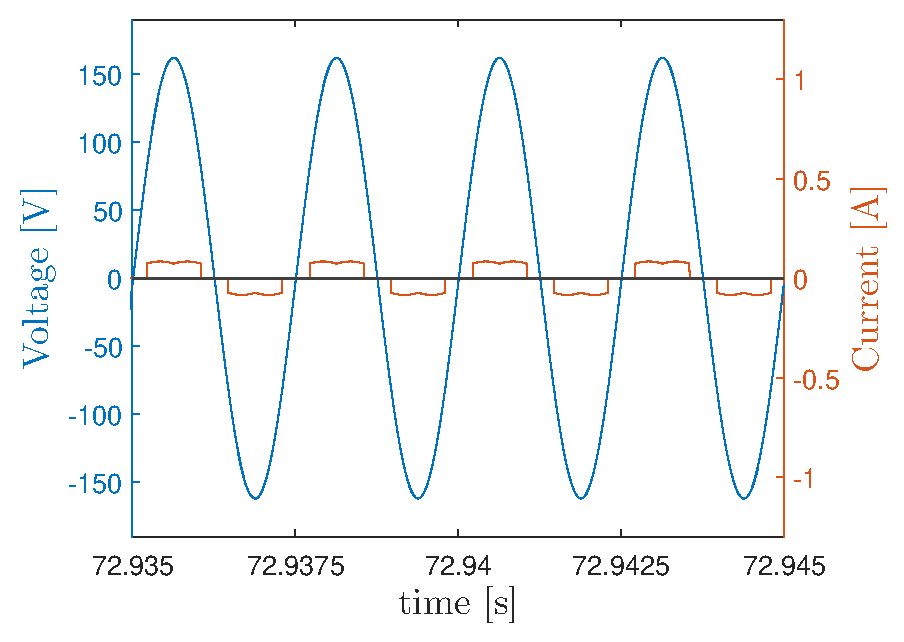
\includegraphics[width=0.4\textwidth]{Figures/artigo_unfilt_1.eps}
	\caption{}
	\label{fig:artigo_unfilt_1.eps}
\end{figure}

\begin{figure}[!b] %
	\centering
	\includegraphics[width=0.4\textwidth]{Figures/artigo_unfilt_2.eps}
	\caption{}
	\label{fig:artigo_unfilt_2.eps}
\end{figure}

\begin{figure}[!b] %
	\centering
	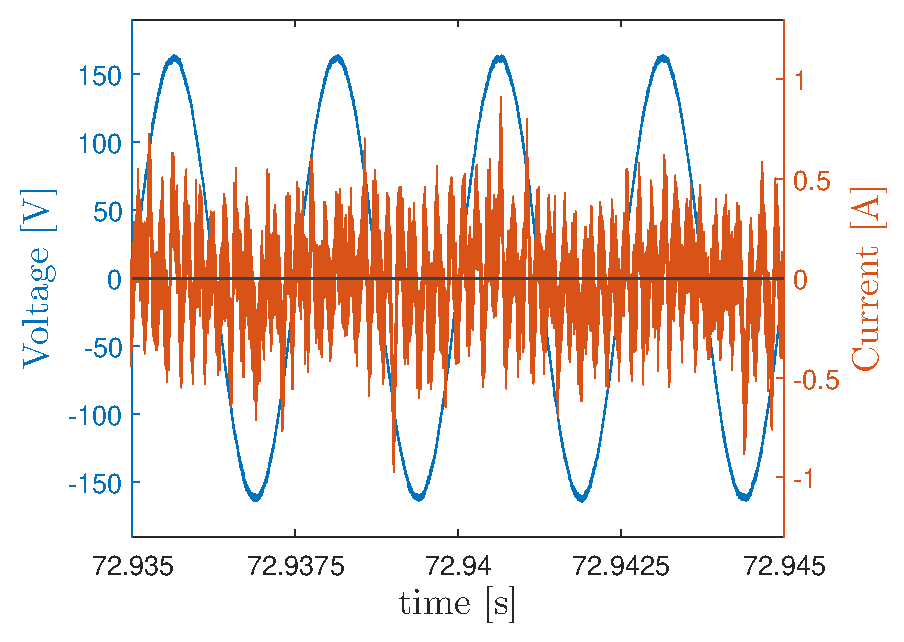
\includegraphics[width=0.4\textwidth]{Figures/artigo_filt_1.eps}
	\caption{}
	\label{fig:artigo_filt_1.eps}
\end{figure}

\begin{figure}[!b] %
	\centering
	\includegraphics[width=0.4\textwidth]{Figures/artigo_filt_2.eps}
	\caption{}
	\label{fig:artigo_filt_2.eps}
\end{figure}

\begin{figure}[!b] %
	\centering
	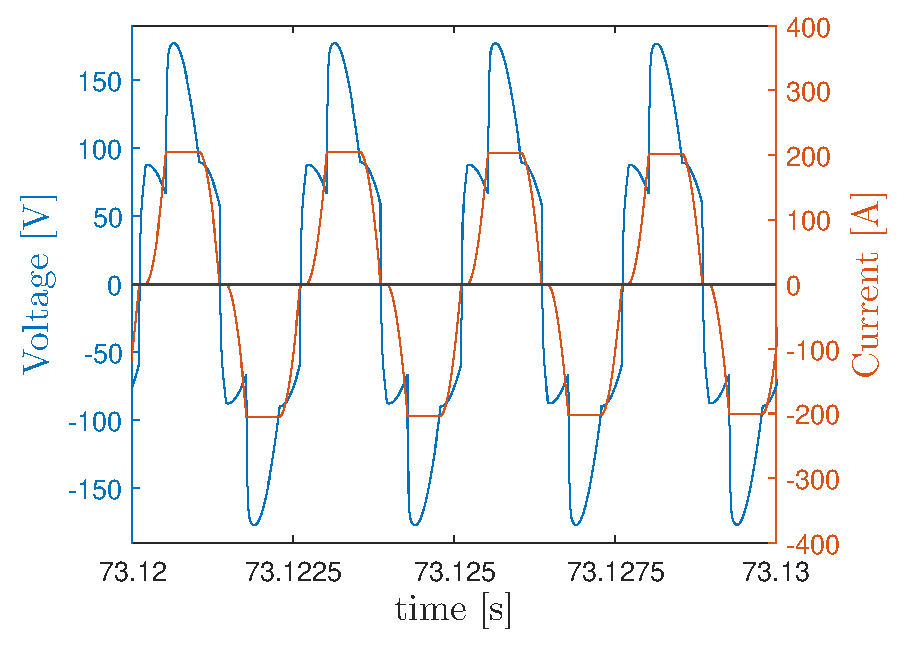
\includegraphics[width=0.4\textwidth]{Figures/artigo_unfilt_3.eps}
	\caption{}
	\label{fig:artigo_unfilt_3.eps}
\end{figure}

\begin{figure}[!b] %
	\centering
	\includegraphics[width=0.4\textwidth]{Figures/artigo_unfilt_4.eps}
	\caption{}
	\label{fig:artigo_unfilt_4.eps}
\end{figure}

\begin{figure}[!b] %
	\centering
	\includegraphics[width=0.4\textwidth]{Figures/artigo_filt_3.eps}
	\caption{}
	\label{fig:artigo_filt_3.eps}
\end{figure}

\begin{figure}[!b] %
	\centering
	\includegraphics[width=0.4\textwidth]{Figures/artigo_filt_4.eps}
	\caption{}
	\label{fig:artigo_filt_4.eps}
\end{figure}

\newpage
\section{Conclusions}

The shunt active filter showed propitious for use in aircraft electrical system to enhance the power quality. The simulation results presented that the active filter response was adequate to high load variation, at the same time its operation maintain the voltage inside the limits defined by the aeronautical standards in terms of harmonic content.

There are some drawbacks when the non-linear loads connected with their respective active filters require low power consumption. In this case, the power quality is slightly degraded, however, not substantially to make the system operate infringing the aeronautical standards.

It should be noticed that even when the loads do not consume power, the set composed by the loads and the filters draw current from the source. This is caused by the energy loss in the filter operation, mainly due to the non-idealities of the switching devices, which is considerable when compared to energy drawn by load operating with low consumption.


\todo[inline]{Traduzir as Figuras}


%Introdução
%=============================================================================================
%\section{INTRODUÇÃO}
%  O texto da introdução deverá apresentar o contexto em que o artigo está inserido, seus objetivos e suas justificativas.
%	O Artigo\footnote{\scriptsize{Mais informações sobre a estruturação dos artigos estão contidas no site: \textcolor[rgb]{0,0,1}{http://eng.embraer.com.br/SETI/SETI/01.html-website/submissao\_artigos.html}.}} deve ser escrito em no máximo 25 páginas, incluindo Texto, Tabelas e/ou Figuras. 
%	A formatação deve seguir tamanho do papel A4, espaçamento entre linhas Simples, formatação do texto Justificado e margens superior, esquerda e direita de 25 mm e inferior 20 mm  (conforme modelo).
%	A língua oficial do congresso é o Português, entretanto serão aceitos artigos em Inglês. Porém, as apresentações deverão ser realizadas em Português. 
%	Os artigos devem ser rigorosamente formatados de acordo com estas instruções.
%
%%Metodologia
%%=============================================================================================
%\section{METODOLOGIA}
%Indicar sucintamente a metodologia utilizada no desenvolvimento do artigo.
%
%%Resultados
%%=============================================================================================
%\section{RESULTADOS}
%Apresentar os principais resultados obtidos no trabalho, podendo ser utilizados gráficos, tabelas e outras ilustrações necessárias à compreensão do tema.
%As equações devem ser apresentadas conforme mostrado pelas Equações \ \ref{e:newton} e \ \ref{e:eq2}.
%
%\begin{equation}
%		\label{e:newton}
%		F=m\alpha
%\end{equation}
%
%\begin{equation}
%		\label{e:eq2} % Este label sera usado para referenciar a equação em algum(s) ponto(s) do texto
%		B=\mu_{0}.(H+M)	
%\end{equation}
%
%As figuras devem ser referenciadas seqüencialmente na parte inferior das mesmas, seguidas do título e centralizadas, como mostrado na Figura \ \ref{figuraAEIOU}. É importante que a figura esteja legível. 
%
%\begin{figure}[htbp!]
%		\centering
%		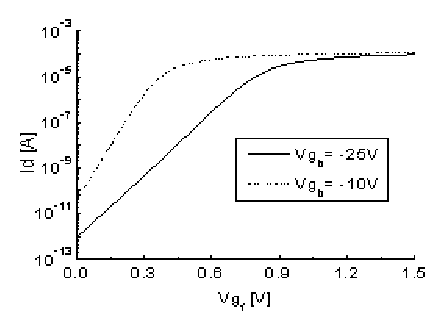
\includegraphics[width=0.5\textwidth]{./figs/Figura1.eps}
%		\caption{Título}
%		\label{figuraAEIOU}	% Usado para referenciar a figura em algum(s) ponto(s) do texto
%\end{figure}
%
%As tabelas devem ser referenciadas seqüencialmente na parte superior das mesmas, seguidas do titulo, como mostrado na Tabela \ \ref{tabelaUOIEA}. O texto da mesma deve ser centralizado.
%
%\begin{table}
%		\centering
%		\begin{tabular}{|c|c|c|c|}\hline
%							& Flaps & Actual & Stage 3 \\ 
%							& Setting & Noise Levels & (EPNdB)  \\
%							&         & (EPNdB)      &          \\ \hline
%			Flyover & 1 & 83.6  & 89.2 \\ \hline
%			Lateral & 1 & 92.6  & 95.3 \\ \hline
%			Approach & 6 & 92.5  & 99.2 \\ \hline
%		\end{tabular}
%		\caption{Título}
%		\label{tabelaUOIEA}
%\end{table}

%Comentários e Conclusões
%%=============================================================================================
%\section{COMENTÁRIOS E CONCLUSÕES}
%Destacar as principais contribuições do autor e indicar, de forma objetiva, as conclusões obtidas.
%
%\vspace{\baselineskip} % Comando para saltar linha (não precisa ter no Artigo final)
%\vspace{\baselineskip} % Comando para saltar linha (não precisa ter no Artigo final)
%
%\underline{\textbf{Referências:}}As referências devem ser indicadas ao longo do texto no formato Schutz (1997) ou (SCHUTZ, 1997) e descritas no final do artigo. Devem ser listados apenas os artigos mencionados no texto, em ordem alfabética do sobrenome, pelo primeiro autor. 
%
%A ordem dos itens em cada referência deve obedecer aos exemplos a seguir.
%\underline{Exemplos:}


%Referências bibliográficas
%=============================================================================================
\clearpage %Para que a parte das referências comece em uma nova página
%\bibliographystyle{apalike}

 \bibliographystyle{abbrvnat}
 \bibliography{Parts/bibliography}
%\setcitestyle{authoryear,open={((},close={))}}
 
%\begin{thebibliography}{50}% maximum number of references (for label width)
%			\bibitem{schutz:1997} SCHUTZ, E. \textbf{Reengenharia mental: reeducação de hábitos e programação de metas}. Florianópolis: Insular, 1997. ({\textbf{Exemplo de livro}})
%			\bibitem{williams:1950} WILLIAMS, J. W. \textbf{Flow measurement}. In: ROUSE, H. (org.). \textbf{Engineering hydraulics.}. New York: John Wiley \& Sons, 1950. p. 229-309. ({\textbf{Exemplo de capítulo de livro}})
%			\bibitem{cup:2003} CIENCIA E OPINIAO. Curitiba: Centro Universitário Positivo. 2003. ({\textbf{Exemplo de periódico}})
%			\bibitem{tozzi:2004} TOZZI, M.; OTA, J.  \textbf{Vertedouro em degraus}. Revista da Vinci, Curitiba, v.1, n.1, p. 9-28, 2004. ({\textbf{Exemplo de artigo de periódico}})
%			\bibitem{veiga:2001} VEIGA, B. V.  \textbf{Modelagem computacional do processo de eutrofização de aplicação de um modelo de balanço de nutrientes a reservatórios da região metropolitana de Curitiba}. Curitiba, 140 p., 2001. Dissertação (Mestrado) – Universidade Federal do Paraná. ({\textbf{Exemplo de monografia, dissertação e tese}})
%			\bibitem{arcdesign:2004} ARC DESIGN. \textbf{Mestres da Arquitetura:} Oscar Niemeyer. São Paulo: Quadrifoglio, n. 35, mar. - abril, 2004. ({\textbf{Exemplo de publicações periódicas consideradas em parte (suplementos, fascículos, números especiais) }})
%			\bibitem{moreira:2004} MOREIRA, T. \textbf{Debate sobre software livre chega ao celular}. Valor Econômico, São Paulo, 04 out. 2004. p. B4. ({\textbf{Exemplo de artigo de jornal}})
%			\bibitem{yoshida:1996} YOSHIDA, S.; VENDRAMIN, J.C.; OLIVEIRA C. \textbf{Tratamento térmico em matrizes de forjaria em prensas de martelo: como aumentar a vida útil}. In: SEMINÁRIO NACIONAL DE FORJAMENTO, 16., Porto Alegre. Anais... Porto Alegre: UFRGS – Centro de Tecnologia, 1996. p. 29-39 ({\textbf{Exemplo de artigo de jornal}})
%			\bibitem{moura:2009} MOURA, G. C. de M. Citação de referências e documentos eletrônicos. Disponível em: \textcolor[rgb]{0,0,1}{http://www.elogica.com.br/users/gmoura/refere.html} Acesso em: 07/01/2009 as 14:00hs. ({\textbf{Exemplo de internet}})
%\end{thebibliography}



\end{document}

